%!TEX program = xelatex
%!TEX TS-program = xelatex
%!TEX encoding = UTF-8 Unicode

\documentclass[12pt, a4paper]{article}
\usepackage{CJKutf8}
\usepackage{graphicx}
\usepackage{subfigure}
\usepackage{listings}
\usepackage[colorlinks,linkcolor=blue]{hyperref}
\usepackage{ulem}
\usepackage{xcolor}
\usepackage{caption2}
\usepackage{amssymb}
\usepackage{indentfirst} % 中文段落首行缩进
\setlength{\parskip}{1em}
\renewcommand{\figurename}{图} % 将图表的标题设置为中文“图”

\title{第十五·蜈蚣博弈 · 直觉倒推存在致命缺陷}
\author{hoochanlon}
\date{\today}

\begin{document}
	\begin{CJK*}{UTF8}{gbsn}
		\maketitle

        \clearpage
        \section{猜数字游戏}
        每个人写一个介于1-100的自然数,求出所有数字的平均数,那么如果某个同学写的这个数,如果某个同学写出这些平均数的1/2,那么就赢的获胜。
        \begin{itemize}
            \item $\geq 50$ 你是别人眼中的傻瓜(捣乱的)。
            \item 25 左右~你把所有听课的同学当傻瓜。
            \item 12-25 你自己不傻,并且也知道别人也不傻。
            \item 6-13 你知道别人知道你不傻。
            \item 1 你百分百不可能胜出,因为你想多了。(除非1是共同知识)
            \end{itemize}

            \begin{figure}[htbp]
                \centering
                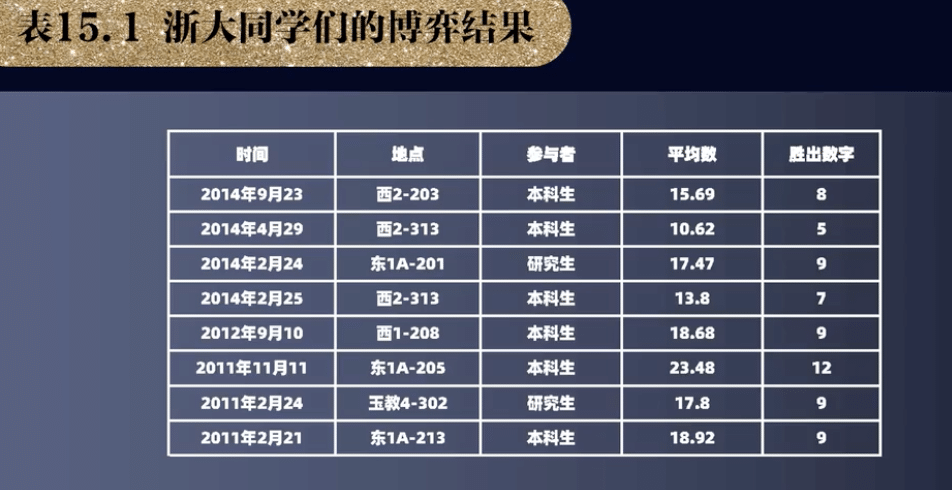
\includegraphics[width=1\textwidth]{./figures/catch2023-07-31-21.01.04.png}
                \caption{博弈结果}
            \end{figure}
            数字游戏结果体现参与者的平均思考深度,一般而言人类的平均思维深度是$1.5\sim2$之间。不同职业之间的思维深度是有明显差异的。

            \section{蜈蚣博弈}
            在蜈蚣博弈中,博弈双方轮流进行策略行为选择。比如股票,股票不断往上涨,只要大家将这个游戏不断玩下去就能一直往上涨,直到游戏结束为止,
            提前买进的获利,最后买进的套牢。

            \subsection{短蜈蚣博弈}
            扔钱游戏,一开始扔50,拒绝的人获得40,接受的人获得10块;但如果两人合作,第二轮开始扔100,拒绝的人获得80,接受的人获得20块。
            第三轮开始扔200,拒绝的人获得160,接受的人获得40块。以此类推,每一轮都是上一轮的两倍。如果一直合作,那么最后一轮的时候,拒绝的人获得$40\times2^{n-1}$。
            \begin{figure}[htbp]
                \centering
                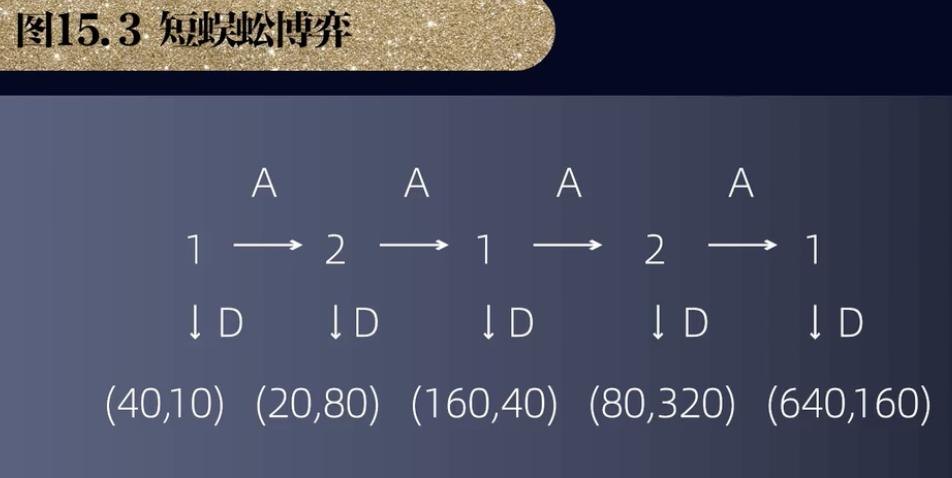
\includegraphics[width=1\textwidth]{./figures/catch2023-08-01-00.08.36.png}
                \caption{蜈蚣模型}
            \end{figure}
            第一个人在最后的800块不得不结束游戏,但第二个人可以在第三步选择不合作。最大的特点,合则双赢,不合则单赢。散户在庄家出货之前卖掉,
            但庄家也不傻,发现散户提前出货,直接再把股票往上拉,要么就在散户出货之前更早出货。\par

            蜈蚣博弈很容易出现自我实现的预言,也称罗森塔尔效应。参与者基于对他人的预期,做出自己的行为选择,而其行为选择又会影响到别人的预期,
            成为别人的行为选择,最终决定博弈的结果。比方说,在股市中如果预期跌,就抢先卖出,一起跌。

            \subsection{博傻理论内涵}
            所有投机行为的关键就是判断价格变化的趋势,选择做多就是你相信还有人愿意用更高的价格,来买你的东西。做空就是你相信还有人愿意用更低的价格。
            博傻理论是指在资本市场中(如股票、期货市场)人们之所以完全不管某个东西的真实价值而愿意花高价购买,是因为他们预期会有一个更大的笨蛋会花更高的价格从他们那把它买走。
            比如交易员将沙丁鱼罐头越买越贵,发现沙丁鱼臭了,罐头只是用来交易的,并不是用来吃的。

            \section{结论}
            一个就是你不要成为别人眼中的傻瓜,第二你也不要把别人来当傻瓜,还有就是有时聪明反被聪明误。


    \end{CJK*}
\end{document}
